\documentclass[11pt,a4paper]{report}
\usepackage[textwidth=37em,vmargin=30mm]{geometry}
\usepackage{calc,xunicode,amsmath,amssymb,paralist,enumitem,tabu,booktabs,datetime2,xeCJK,xeCJKfntef,listings}
\usepackage{tocloft,fancyhdr,tcolorbox,xcolor,graphicx,eso-pic,xltxtra,xelatexemoji}

\newcommand{\envyear}[0]{2025}
\newcommand{\envdatestr}[0]{2025-02-26}
\newcommand{\envfinaldir}[0]{webdb/2025/20250226/final}

\usepackage[hidelinks]{hyperref}
\hypersetup{
    colorlinks=false,
    pdfpagemode=FullScreen,
    pdftitle={Web Digest - \envdatestr}
}

\setlength{\cftbeforechapskip}{10pt}
\renewcommand{\cftchapfont}{\rmfamily\bfseries\large\raggedright}
\setlength{\cftbeforesecskip}{2pt}
\renewcommand{\cftsecfont}{\sffamily\small\raggedright}

\setdefaultleftmargin{2em}{2em}{1em}{1em}{1em}{1em}

\usepackage{xeCJK,xeCJKfntef}
\xeCJKsetup{PunctStyle=plain,RubberPunctSkip=false,CJKglue=\strut\hskip 0pt plus 0.1em minus 0.05em,CJKecglue=\strut\hskip 0.22em plus 0.2em}
\XeTeXlinebreaklocale "zh"
\XeTeXlinebreakskip = 0pt


\setmainfont{Brygada 1918}
\setromanfont{Brygada 1918}
\setsansfont{IBM Plex Sans}
\setmonofont{JetBrains Mono NL}
\setCJKmainfont{Noto Serif CJK SC}
\setCJKromanfont{Noto Serif CJK SC}
\setCJKsansfont{Noto Sans CJK SC}
\setCJKmonofont{Noto Sans CJK SC}

\setlength{\parindent}{0pt}
\setlength{\parskip}{8pt}
\linespread{1.15}

\lstset{
	basicstyle=\ttfamily\footnotesize,
	numbersep=5pt,
	backgroundcolor=\color{black!5},
	showspaces=false,
	showstringspaces=false,
	showtabs=false,
	tabsize=2,
	captionpos=b,
	breaklines=true,
	breakatwhitespace=true,
	breakautoindent=true,
	linewidth=\textwidth
}






\newcommand{\coverpic}[2]{
    % argv: itemurl, authorname
    Cover photo by #2~~(\href{#1}{#1})
}
\newcommand{\makeheader}[0]{
    \begin{titlepage}
        % \newgeometry{hmargin=15mm,tmargin=21mm,bmargin=12mm}
        \begin{center}
            
            \rmfamily\scshape
            \fontspec{BaskervilleF}
            \fontspec{Old Standard}
            \fontsize{59pt}{70pt}\selectfont
            WEB\hfill DIGEST
            
            \vfill
            % \vskip 30pt
            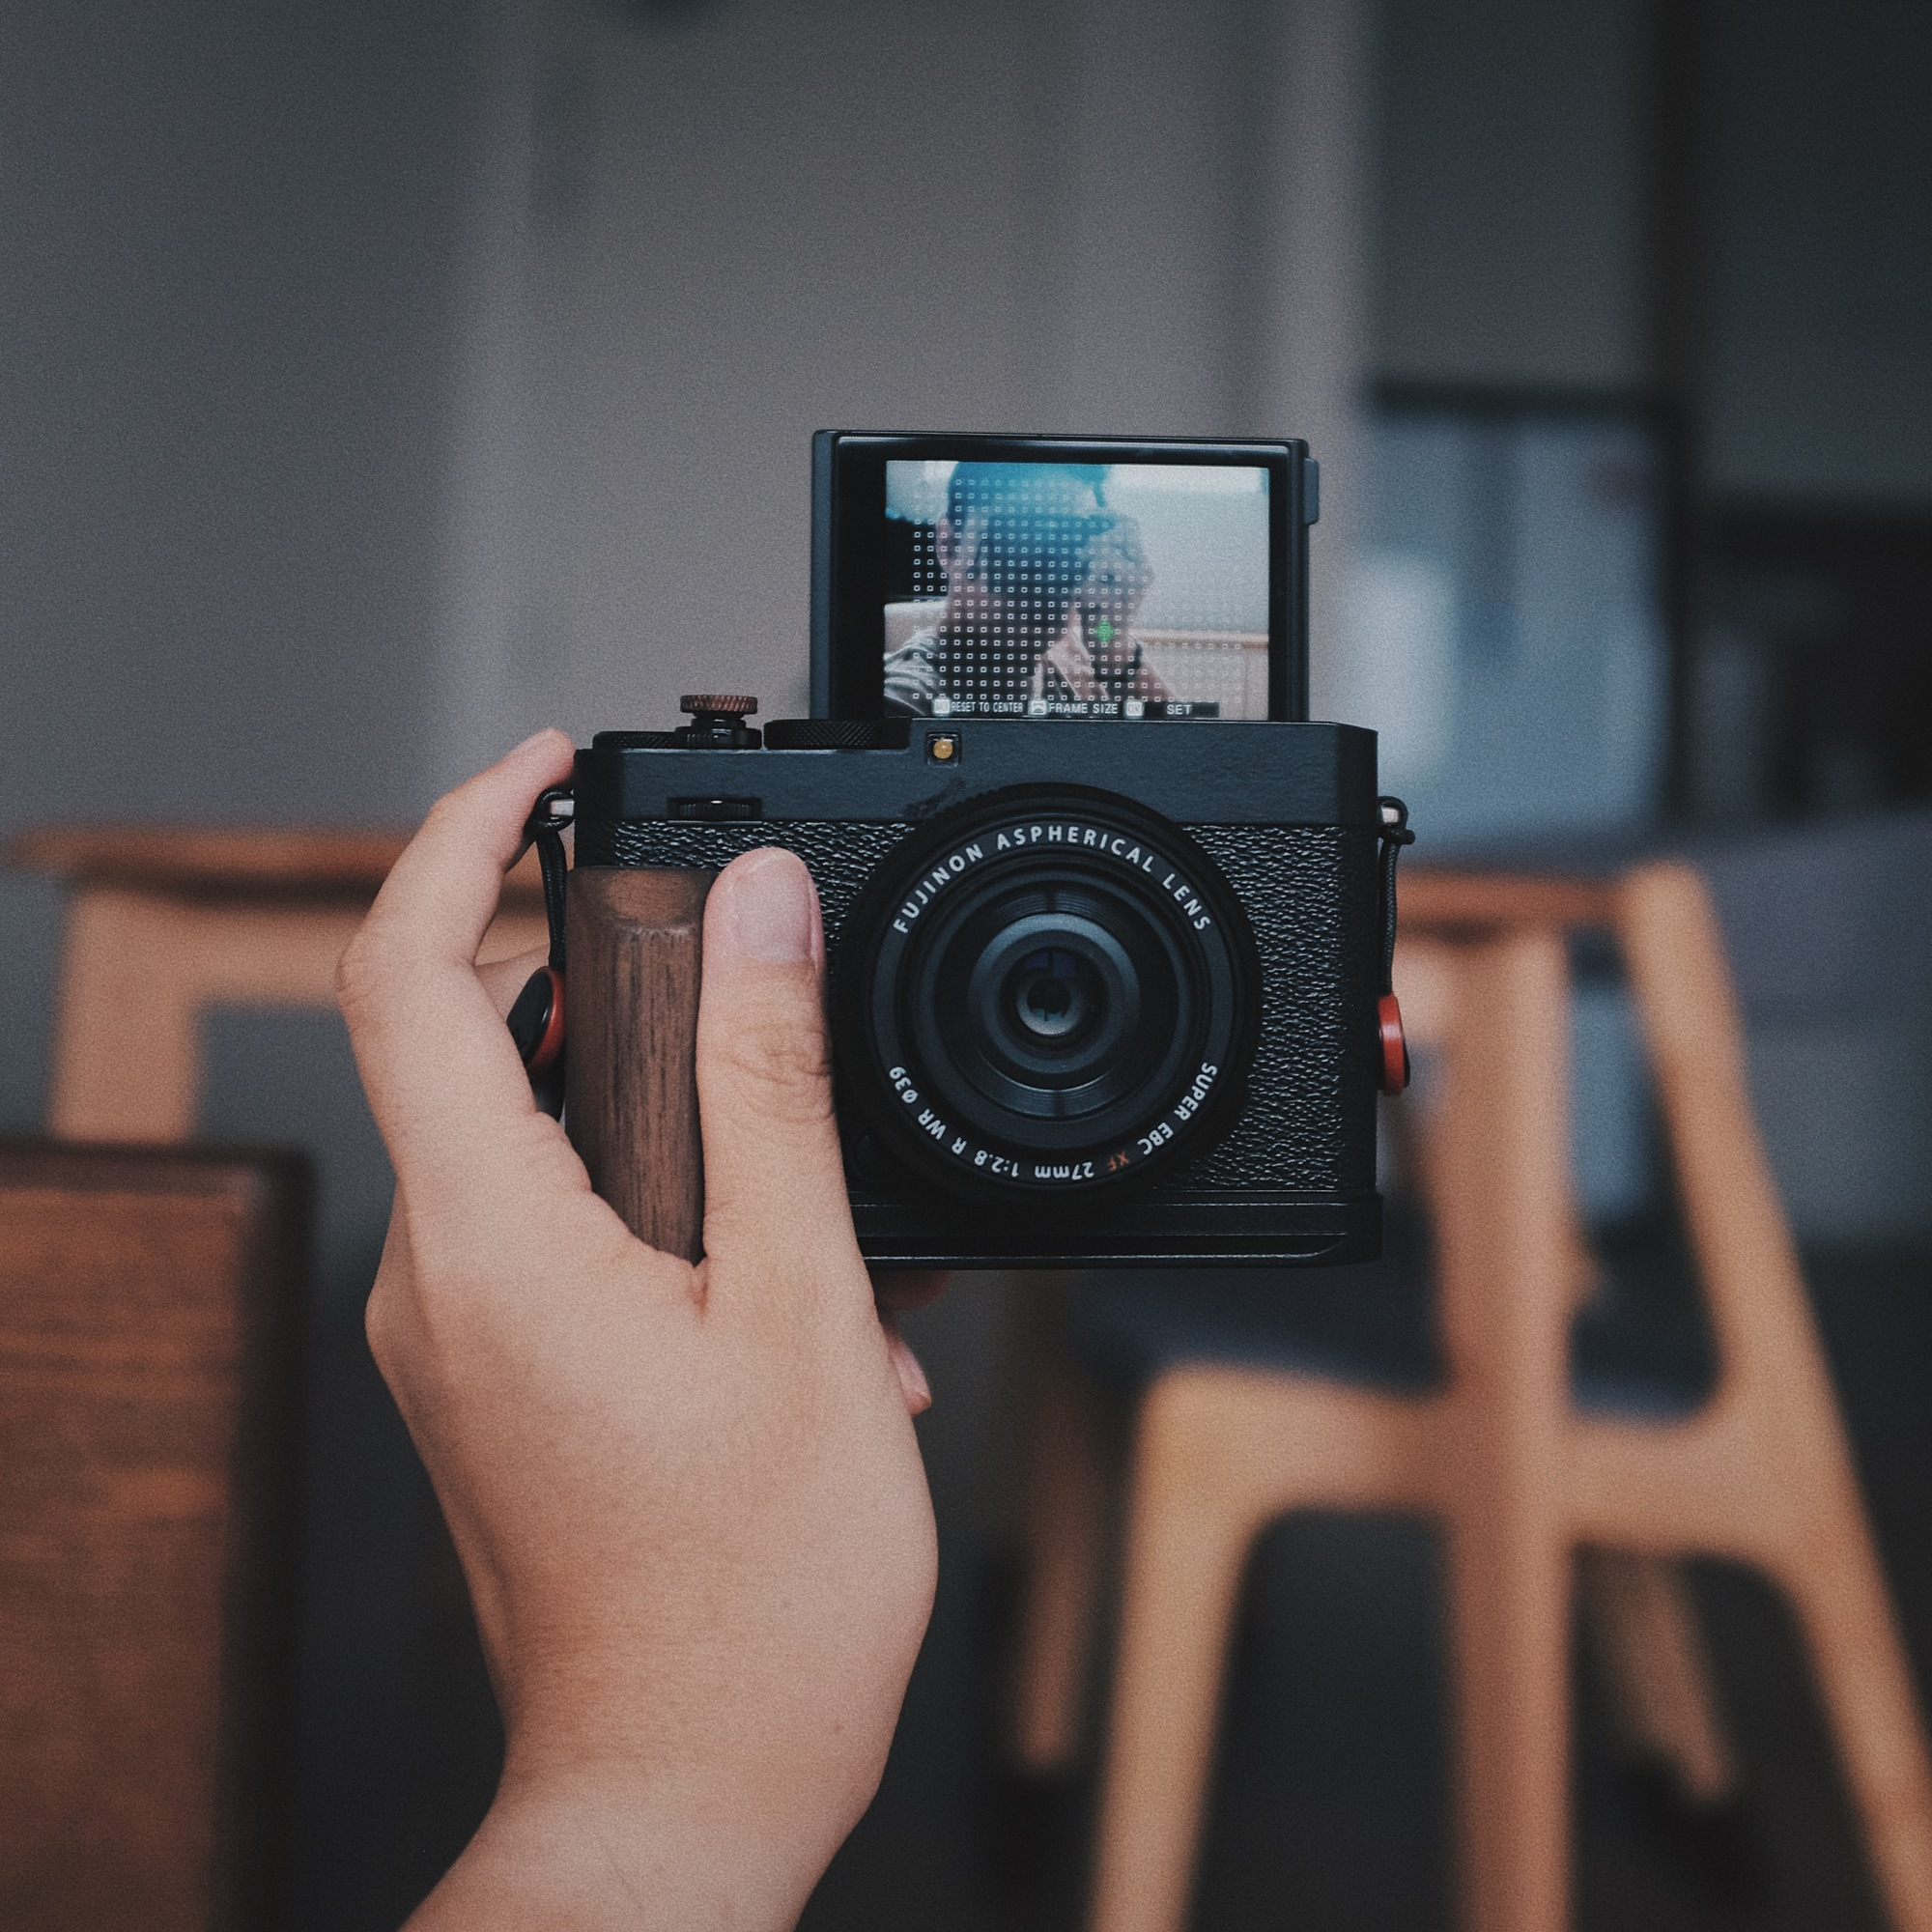
\includegraphics[width=\linewidth]{\envfinaldir/coverpic-prod.jpg}\par
            % \vskip 30pt
            \vfill

            \normalsize\rmfamily\scshape
            \copyright{} The Web Digest Project \hfill\large \envdatestr
        \end{center}
    \end{titlepage}
    % \restoregeometry
}
\newcommand{\simplehref}[1]{%
    \textcolor{blue!80!green}{\href{#1}{#1}}%
}
\renewcommand{\contentsname}{\center\Huge\sffamily\bfseries Contents\par\vskip 20pt}
\newcounter{ipartcounter}
\setcounter{ipartcounter}{0}
\newcommand{\ipart}[1]{
    % \vskip 20pt
    \clearpage
    \stepcounter{ipartcounter}
    \phantomsection
    \addcontentsline{toc}{chapter}{#1}
    % \begin{center}
    %     \Huge
    %     \sffamily\bfseries
    %     #1
    % \end{center}
    % \vskip 20pt plus 7pt
}
\newcounter{ichaptercounter}
\setcounter{ichaptercounter}{0}
\newcommand{\ichapter}[1]{
    % \vskip 20pt
    \clearpage
    \stepcounter{ichaptercounter}
    \phantomsection
    \addcontentsline{toc}{section}{\numberline{\arabic{ichaptercounter}}#1}
    \begin{center}
        \Huge
        \sffamily\bfseries
        #1
    \end{center}
    \vskip 20pt plus 7pt
}
\newcommand{\entrytitlefont}[1]{\subsection*{\raggedright\Large\sffamily\bfseries#1}}
\newcommand{\entryitemGeneric}[2]{
    % argv: title, url
    \parbox{\linewidth}{
        \entrytitlefont{#1}\par\vskip 5pt
        \footnotesize\ttfamily\mdseries
        \simplehref{#2}
    }\vskip 11pt plus 11pt minus 1pt
}
\newcommand{\entryitemGithub}[3]{
    % argv: title, url, desc
    \parbox{\linewidth}{
        \entrytitlefont{#1}\par\vskip 5pt
        \footnotesize\ttfamily\mdseries
        \simplehref{#2}\par\vskip 5pt
        \small\rmfamily\mdseries#3
    }\vskip 11pt plus 11pt minus 1pt
}
\newcommand{\entryitemAp}[3]{
    % argv: title, url, desc
    \parbox{\linewidth}{
        \entrytitlefont{#1}\par\vskip 5pt
        \footnotesize\ttfamily\mdseries
        \simplehref{#2}\par\vskip 5pt
        \small\rmfamily\mdseries#3
    }\vskip 11pt plus 11pt minus 1pt
}
\newcommand{\entryitemHackernews}[3]{
    % argv: title, hnurl, rawurl
    % \parbox{\linewidth}{
    %     \entrytitlefont{#1}\par\vskip 5pt
    %     \footnotesize\ttfamily\mdseries
    %     \simplehref{#3}\par
    %     \textcolor{black!50}{\href{#2}{#2}}
    % }\vskip 11pt plus 11pt minus 1pt
    \begin{minipage}{\linewidth}
            \entrytitlefont{#1}\par\vskip 5pt
            \footnotesize\ttfamily\mdseries
            \simplehref{#3}\par
            \textcolor{black!50}{\href{#2}{#2}}
    \end{minipage}\par\vskip 11pt plus 11pt minus 1pt
}







\begin{document}

\makeheader

\tableofcontents\clearpage




\ipart{Developers}
\ichapter{Hacker News}
\entryitemTwoLinks{Framework's first desktop is a strange–but unique–mini ITX gaming PC}{https://news.ycombinator.com/item?id=43176314}{https://arstechnica.com/gadgets/2025/02/framework-known-for-upgradable-laptops-intros-not-particularly-upgradable-desktop/}

\entryitemTwoLinks{I Went to SQL Injection Court}{https://news.ycombinator.com/item?id=43175628}{https://sockpuppet.org/blog/2025/02/09/fixing-illinois-foia/}

\entryitemTwoLinks{The XB-70 (2019)}{https://news.ycombinator.com/item?id=43175315}{http://codex99.com/photography/the-xb70.html}

\entryitemTwoLinks{'Hey Number 17 '}{https://news.ycombinator.com/item?id=43175023}{https://www.404media.co/email/b7eb2339-2ea1-4a37-96cc-a360494c214c/}

\entryitemTwoLinks{Hard problems that reduce to document ranking}{https://news.ycombinator.com/item?id=43174910}{https://noperator.dev/posts/document-ranking-for-complex-problems/}

\entryitemTwoLinks{Hyperspace}{https://news.ycombinator.com/item?id=43173462}{https://hypercritical.co/2025/02/25/hyperspace}

\entryitemTwoLinks{Launch HN: Browser Use (YC W25) – open-source web agents}{https://news.ycombinator.com/item?id=43173378}{https://github.com/browser-use/browser-use}

\entryitemTwoLinks{DeepSearcher: A local open-source Deep Research}{https://news.ycombinator.com/item?id=43172338}{https://milvus.io/blog/introduce-deepsearcher-a-local-open-source-deep-research.md}

\entryitemTwoLinks{ChatGPT Saved My Life (no, seriously, I'm writing this from the ER)}{https://news.ycombinator.com/item?id=43171639}{https://hardmodefirst.xyz/chatgpt-saved-my-life-no,-seriously,-im-writing-this-from-the-er}

\entryitemTwoLinks{Unknown illness kills over 50 in Congo with hours between symptoms and death}{https://news.ycombinator.com/item?id=43171371}{https://apnews.com/article/congo-mystery-unknown-illness-cd8b1fdcb3b2ed032968b2c6044dc6db}

\entryitemTwoLinks{DOGE will use AI to assess the responses of federal workers}{https://news.ycombinator.com/item?id=43171265}{https://www.nbcnews.com/politics/doge/federal-workers-agencies-push-back-elon-musks-email-ultimatum-rcna193439}

\entryitemTwoLinks{Embedding Python in Elixir, it's fine}{https://news.ycombinator.com/item?id=43171239}{https://dashbit.co/blog/running-python-in-elixir-its-fine}

\entryitemTwoLinks{Signal to leave Sweden if backdoor law passes}{https://news.ycombinator.com/item?id=43171205}{https://swedenherald.com/article/signals-ceo-then-were-leaving-sweden}

\entryitemTwoLinks{A Defense of Weird Research}{https://news.ycombinator.com/item?id=43171002}{https://asteriskmag.com/issues/09/a-defense-of-weird-research}

\entryitemTwoLinks{Tell HN: Y Combinator backing AI company to abuse factory workers}{https://news.ycombinator.com/item?id=43170850}{https://news.ycombinator.com/item?id=43170850}

\entryitemTwoLinks{Chicory: A JVM native WebAssembly runtime}{https://news.ycombinator.com/item?id=43170545}{https://chicory.dev/}

\entryitemTwoLinks{Tesla sales in Europe down 45\% in January}{https://news.ycombinator.com/item?id=43170090}{https://www.ft.com/content/cdd0b5c8-2703-4fd4-9ebf-26087cac8523}

\entryitemTwoLinks{Awesome DeepSeek Integrations}{https://news.ycombinator.com/item?id=43169827}{https://github.com/deepseek-ai/awesome-deepseek-integration}

\entryitemTwoLinks{How Core Git Developers Configure Git}{https://news.ycombinator.com/item?id=43169435}{https://blog.gitbutler.com/how-git-core-devs-configure-git/}

\entryitemTwoLinks{What would happen if we didn't use TCP or UDP?}{https://news.ycombinator.com/item?id=43169103}{https://github.com/Hawzen/hdp}\ichapter{Phoronix}
\entryitemGeneric{\hskip 0pt{}Christoph Hellwig Steps Down From One Of His Kernel Roles Following Rust Drama}{https://www.phoronix.com/news/Hellwig-DMA-Helpers-Removed}

\entryitemGeneric{\hskip 0pt{}AMD Ryzen 9000 vs. Intel Core Ultra Arrow Lake On Linux For Q1-2025 In ~400 Benchmarks}{https://www.phoronix.com/review/ryzen9000-core-ultra-linux613}

\entryitemGeneric{\hskip 0pt{}Eight New Security Vulnerabilities Reported Against The X.Org Server \& XWayland}{https://www.phoronix.com/news/Eight-New-X.Org-Security-Issues}

\entryitemGeneric{\hskip 0pt{}Rust-Written Zlib-rs Is Not Only Safer But Now Outperforming Zlib C Implementations}{https://www.phoronix.com/news/Zlib-rs-0.4.2}

\entryitemGeneric{\hskip 0pt{}Linux 6.15 Intel Xe Driver Enabling PXP HWDRM, Survivability Mode \& GPU + VRAM Temperatures}{https://www.phoronix.com/news/Intel-Xe-Linux-6.15-First}

\entryitemGeneric{\hskip 0pt{}GNOME 48 Mutter Merges Wayland's wp\_color\_management\_v1 Support}{https://www.phoronix.com/news/GNOME-wp\_color\_management\_v1}

\entryitemGeneric{\hskip 0pt{}MythTV 35 Released For This Once Widely-Used Open-Source DVR/PVR Software}{https://www.phoronix.com/news/MythTV-35-Released}

\entryitemGeneric{\hskip 0pt{}Armbian 25.2 Released With New Boards Supported, Kernel Upgrades}{https://www.phoronix.com/news/Armbian-25.2-Released}

\entryitemGeneric{\hskip 0pt{}Canonical Rolling Out Improved CLA Process For Ubuntu Contributions}{https://www.phoronix.com/news/Canonical-Better-CLA-Process}\ichapter{Dribbble}
\entryitemGeneric{\hskip 0pt{}Letter a}{https://dribbble.com/shots/25680095-Letter-a}

\entryitemGeneric{\hskip 0pt{}auren - logo design}{https://dribbble.com/shots/25681046-auren-logo-design}

\entryitemGeneric{\hskip 0pt{}Cardi C}{https://dribbble.com/shots/25678066-Cardi-C}

\entryitemGeneric{\hskip 0pt{}R}{https://dribbble.com/shots/25673587-R}

\entryitemGeneric{\hskip 0pt{}Unused Geometric Fox}{https://dribbble.com/shots/25677006-Unused-Geometric-Fox}

\entryitemGeneric{\hskip 0pt{}Triceratops Dino}{https://dribbble.com/shots/25676249-Triceratops-Dino}

\entryitemGeneric{\hskip 0pt{}Fitme home landing page}{https://dribbble.com/shots/25674639-Fitme-home-landing-page}

\entryitemGeneric{\hskip 0pt{}Illustrated Icons - American Home Shield}{https://dribbble.com/shots/25666386-Illustrated-Icons-American-Home-Shield}

\entryitemGeneric{\hskip 0pt{}Tiger Style}{https://dribbble.com/shots/25676567-Tiger-Style}

\entryitemGeneric{\hskip 0pt{}Logo Tip 002. Rhythm in Logo Design}{https://dribbble.com/shots/25674872-Logo-Tip-002-Rhythm-in-Logo-Design}

\entryitemGeneric{\hskip 0pt{}The Business}{https://dribbble.com/shots/25676385-The-Business}

\entryitemGeneric{\hskip 0pt{}Cute Dinosaur}{https://dribbble.com/shots/25671549-Cute-Dinosaur}

\entryitemGeneric{\hskip 0pt{}BNPL service}{https://dribbble.com/shots/25664920-BNPL-service}

\entryitemGeneric{\hskip 0pt{}Wolf Creek Golf Club}{https://dribbble.com/shots/25664483-Wolf-Creek-Golf-Club}

\entryitemGeneric{\hskip 0pt{}Business illustration set}{https://dribbble.com/shots/25661493-Business-illustration-set}

\entryitemGeneric{\hskip 0pt{}b}{https://dribbble.com/shots/25663031-b}

\entryitemGeneric{\hskip 0pt{}ProAWS Logo Design}{https://dribbble.com/shots/25661915-ProAWS-Logo-Design}

\entryitemGeneric{\hskip 0pt{}Form Golf ID}{https://dribbble.com/shots/25660910-Form-Golf-ID}

\entryitemGeneric{\hskip 0pt{}Shooting Ladybug - Make a wish! Nagare Mushi}{https://dribbble.com/shots/25659882-Shooting-Ladybug-Make-a-wish-Nagare-Mushi}

\entryitemGeneric{\hskip 0pt{}Puzzle Fintech Website Design [Case Study]}{https://dribbble.com/shots/25478108-Puzzle-Fintech-Website-Design-Case-Study}

\entryitemGeneric{\hskip 0pt{}Pendleton Whisky}{https://dribbble.com/shots/25650439-Pendleton-Whisky}

\entryitemGeneric{\hskip 0pt{}Sugar Glider Logo}{https://dribbble.com/shots/25653559-Sugar-Glider-Logo}

\entryitemGeneric{\hskip 0pt{}Form Golf Wordmark}{https://dribbble.com/shots/25655786-Form-Golf-Wordmark}

\entryitemGeneric{\hskip 0pt{}Logo Design for Ai Assistant Part One}{https://dribbble.com/shots/25652926-Logo-Design-for-Ai-Assistant-Part-One}


\ipart{Developers~~~~(zh-Hans)}
\ichapter{Solidot}
\entryitemGeneric{\hskip 0pt{}火星上的古代海滩显示它曾经有海洋}{https://www.solidot.org/story?sid=80649}

\entryitemGeneric{\hskip 0pt{}未知疾病在刚果杀死了逾 50 人}{https://www.solidot.org/story?sid=80648}

\entryitemGeneric{\hskip 0pt{}短期摄入大量高热量饮食会改变大脑模式}{https://www.solidot.org/story?sid=80647}

\entryitemGeneric{\hskip 0pt{}特斯拉汽车欧洲 1 月销量暴跌 45\%}{https://www.solidot.org/story?sid=80645}

\entryitemGeneric{\hskip 0pt{}Aqualung 2.0 释出}{https://www.solidot.org/story?sid=80644}

\entryitemGeneric{\hskip 0pt{}微软将第 11 代前的英特尔处理器移出 Windows 11 24H2 兼容列表 }{https://www.solidot.org/story?sid=80643}

\entryitemGeneric{\hskip 0pt{}朝鲜黑客如何盗走 15 亿美元加密货币}{https://www.solidot.org/story?sid=80642}

\entryitemGeneric{\hskip 0pt{}Gmail 用 QR 码取代短信验证}{https://www.solidot.org/story?sid=80641}

\entryitemGeneric{\hskip 0pt{}2024 年大气二氧化碳浓度增幅创新高}{https://www.solidot.org/story?sid=80640}

\entryitemGeneric{\hskip 0pt{}中国主要电视机品牌出货量首超韩国}{https://www.solidot.org/story?sid=80639}

\entryitemGeneric{\hskip 0pt{}微软推出广告版 Microsoft Office}{https://www.solidot.org/story?sid=80638}

\entryitemGeneric{\hskip 0pt{}Anthropic 发布混合推理模型 Claude 3.7 Sonnet}{https://www.solidot.org/story?sid=80637}

\entryitemGeneric{\hskip 0pt{}GDC 终身成就奖授予 Sam Lake 先锋奖授予 Lucas Pope}{https://www.solidot.org/story?sid=80636}

\entryitemGeneric{\hskip 0pt{}德国创业公司准备尝试西欧首次轨道发射}{https://www.solidot.org/story?sid=80635}

\entryitemGeneric{\hskip 0pt{}研究发现零工在 2024 年工作时间更长但收入更少}{https://www.solidot.org/story?sid=80634}

\entryitemGeneric{\hskip 0pt{}研究发现用于高尔夫球场的土地超过风能或太阳能}{https://www.solidot.org/story?sid=80633}

\entryitemGeneric{\hskip 0pt{}英伟达证实部分 RTX 50 系列显卡有缺陷}{https://www.solidot.org/story?sid=80632}

\entryitemGeneric{\hskip 0pt{}Starlink 面临越来越多的竞争}{https://www.solidot.org/story?sid=80631}

\entryitemGeneric{\hskip 0pt{}韦伯望远镜观测到银河黑洞非常活跃}{https://www.solidot.org/story?sid=80630}

\entryitemGeneric{\hskip 0pt{}马斯克呼吁尽可能快的将国际空间站脱离轨道}{https://www.solidot.org/story?sid=80629}\ichapter{V2EX}
\entryitemGeneric{\hskip 0pt{}[信息安全] 关于 iOS18.3.1 剪贴板被访问时的问题}{https://www.v2ex.com/t/1114231}

\entryitemGeneric{\hskip 0pt{}[Java] 使用 Java 写了一版 LangChain,想听听大家的意见}{https://www.v2ex.com/t/1114230}

\entryitemGeneric{\hskip 0pt{}[问与答] BoltAI 似乎无法设置火山云 api 调用 ?}{https://www.v2ex.com/t/1114227}

\entryitemGeneric{\hskip 0pt{}[问与答] Google 相册怎么恢复回收站里的内容到手机本地?}{https://www.v2ex.com/t/1114226}

\entryitemGeneric{\hskip 0pt{}[问与答] 本人遇到了非常棘手奇怪的关于``注释''ctrl+/ 快捷键失灵?无法绑定?的问题。}{https://www.v2ex.com/t/1114225}

\entryitemGeneric{\hskip 0pt{}[问与答] 手机屏幕绿线}{https://www.v2ex.com/t/1114224}

\entryitemGeneric{\hskip 0pt{}[问与答] 逆向从众?有没有同样不追热点的朋友}{https://www.v2ex.com/t/1114223}

\entryitemGeneric{\hskip 0pt{}[Apple] 黑苹果末路?}{https://www.v2ex.com/t/1114222}

\entryitemGeneric{\hskip 0pt{}[程序员] 想在海外发布一个 saas 程序,后端 Java + MySQL,哪里买服务器最便宜?}{https://www.v2ex.com/t/1114221}

\entryitemGeneric{\hskip 0pt{}[问与答] 有没支持 M1 芯片的 Gewechat docker 镜像}{https://www.v2ex.com/t/1114220}

\entryitemGeneric{\hskip 0pt{}[macOS] Mac mini m4 显示器怎么选?}{https://www.v2ex.com/t/1114219}

\entryitemGeneric{\hskip 0pt{}[酷工作] [校招内推] 三七互娱-开发/策划/运营/美术}{https://www.v2ex.com/t/1114218}

\entryitemGeneric{\hskip 0pt{}[GitHub] 发现 Github 账号上有异常活动,疑似被盗}{https://www.v2ex.com/t/1114217}

\entryitemGeneric{\hskip 0pt{}[酷工作] 远程大模型工作, 10-20 万美金,硅谷公司}{https://www.v2ex.com/t/1114216}

\entryitemGeneric{\hskip 0pt{}[分享创造] 开源 AI 聊天软件 AIdea 2.0 发布:支持 DeepSeek、Claude 3.7 Sonnet 深度思考、联网搜索}{https://www.v2ex.com/t/1114215}

\entryitemGeneric{\hskip 0pt{}[分享创造] 我用 cursor 一小时写了一个 Google SEO API 索引提交油猴脚本}{https://www.v2ex.com/t/1114214}

\entryitemGeneric{\hskip 0pt{}[OpenWrt] passwall 弄不好了!关于 windows edge chrome}{https://www.v2ex.com/t/1114212}

\entryitemGeneric{\hskip 0pt{}[程序员] 牛逼: 30 岁女程序员逆袭, 3 年靠织毛线球赚千万美元}{https://www.v2ex.com/t/1114211}

\entryitemGeneric{\hskip 0pt{}[JavaScript] 本人遇到了非常奇怪的关于``注释''ctrl+/ 快捷键问题,需要大佬们指点一二。}{https://www.v2ex.com/t/1114210}

\entryitemGeneric{\hskip 0pt{}[程序员] 准备跳槽, v 友有什么见过的有意思的有意义的面试题吗,方向后端开发 go 为主。可以是算法, k8s, docker 方面的都行。}{https://www.v2ex.com/t/1114209}

\entryitemGeneric{\hskip 0pt{}[程序员] 2025 年有没有大容量 HDD 推荐}{https://www.v2ex.com/t/1114208}

\entryitemGeneric{\hskip 0pt{}[宽带症候群] 国内 4G 基站现状}{https://www.v2ex.com/t/1114207}

\entryitemGeneric{\hskip 0pt{}[问与答] 我的 Apple account 这是被封了吗?}{https://www.v2ex.com/t/1114206}

\entryitemGeneric{\hskip 0pt{}[程序员] 智能运维实现思路}{https://www.v2ex.com/t/1114205}

\entryitemGeneric{\hskip 0pt{}[NAS] 有没有这样一款能在 Linux 和 windows 之间同步文件夹的软件?}{https://www.v2ex.com/t/1114204}

\entryitemGeneric{\hskip 0pt{}[Apple] 我有歌曲文件,怎么才能让 Apple Music 识别歌曲信息从而显示专辑封面和歌词?}{https://www.v2ex.com/t/1114202}

\entryitemGeneric{\hskip 0pt{}[问与答] 请问高中各地各名校的真题试卷哪里下载?}{https://www.v2ex.com/t/1114199}

\entryitemGeneric{\hskip 0pt{}[程序员] 如何利用大模型增加测试范围及能力}{https://www.v2ex.com/t/1114198}

\entryitemGeneric{\hskip 0pt{}[程序员] 我建了一个微信群,希望大家可以交流出海赚钱的想法}{https://www.v2ex.com/t/1114197}

\entryitemGeneric{\hskip 0pt{}[创业组队] 杭州炸鱼薯条寻创业伙伴}{https://www.v2ex.com/t/1114196}

\entryitemGeneric{\hskip 0pt{}[问与答] hp 笔记本的电池坏了,每次启动 cmos 都报错,有好解决办法吗?}{https://www.v2ex.com/t/1114195}

\entryitemGeneric{\hskip 0pt{}[分享发现] 让游戏再次伟大--- 用 grok3 和 claude3.7 一句话生成街机游戏原型,结果出乎意料!}{https://www.v2ex.com/t/1114194}

\entryitemGeneric{\hskip 0pt{}[生活] 支付宝开始支持绑定美国运通卡}{https://www.v2ex.com/t/1114192}

\entryitemGeneric{\hskip 0pt{}[创业组队] 找个伙伴一起折腾创业}{https://www.v2ex.com/t/1114191}

\entryitemGeneric{\hskip 0pt{}[分享发现] 2025 年将是程序员``终结的开始'' (Beginning of the End)-扎克伯格}{https://www.v2ex.com/t/1114190}

\entryitemGeneric{\hskip 0pt{}[问与答] Google Play 绑定的邮箱收到一封邮件,说每月给我 200 美元,这是真的吗?}{https://www.v2ex.com/t/1114189}

\entryitemGeneric{\hskip 0pt{}[酷工作] [广州-三七互娱-校招] 算法工程师、前端开发工程师(Cocos/UE+AI 方向)、前端开发工程师、数据开发工程师、后端开发工程师}{https://www.v2ex.com/t/1114188}

\entryitemGeneric{\hskip 0pt{}[程序员] [分享] 刚发现 DeepSeek 可以充值了}{https://www.v2ex.com/t/1114187}

\entryitemGeneric{\hskip 0pt{}[分享发现] [邮件评测] Spacemail (Spaceship) (5/10)}{https://www.v2ex.com/t/1114186}

\entryitemGeneric{\hskip 0pt{}[分享创造] 抓取 Claude 及 ChatGPT 对话并保存的脚本}{https://www.v2ex.com/t/1114185}

\entryitemGeneric{\hskip 0pt{}[程序员] 年收入 16w,被嫌弃了}{https://www.v2ex.com/t/1114184}

\entryitemGeneric{\hskip 0pt{}[分享创造] 开源我做的修仙智能体「一念成仙」的底层项目}{https://www.v2ex.com/t/1114183}

\entryitemGeneric{\hskip 0pt{}[VXNA] 申请收录 www.mailer.su}{https://www.v2ex.com/t/1114182}

\entryitemGeneric{\hskip 0pt{}[问与答] ai 生图工具求推荐}{https://www.v2ex.com/t/1114181}

\entryitemGeneric{\hskip 0pt{}[程序员] claude code 的意义是什么?和 cursor 有什么区别?}{https://www.v2ex.com/t/1114180}

\entryitemGeneric{\hskip 0pt{}[推广] JavaGuide | JavaGuide.net 指南 | Java 最强八股文}{https://www.v2ex.com/t/1114179}

\entryitemGeneric{\hskip 0pt{}[问与答] 求助万能的 v 友,想找一个能够沟通翻译相关内容的平台}{https://www.v2ex.com/t/1114178}

\entryitemGeneric{\hskip 0pt{}[程序员] 我录了一期博客,记录一下自己的副业之路,我是怎么开始的。}{https://www.v2ex.com/t/1114177}

\entryitemGeneric{\hskip 0pt{}[问与答] 电脑端有什么播放器支持统计播放音乐的次数?}{https://www.v2ex.com/t/1114176}

\entryitemGeneric{\hskip 0pt{}[问与答] 最近看到一些 app 上架 play 商店需要测试人数的问题}{https://www.v2ex.com/t/1114175}


\ipart{Generic News}







\clearpage
\leavevmode\vfill
\footnotesize

Copyright \copyright{} 2023-2025 Neruthes and other contributors.

This document is published with CC BY-NC-ND 4.0 license.

The entries listed in this newsletter may be copyrighted by their respective creators.

This newsletter is generated by the Web Digest project.

The newsletters are also delivered via Telegram channel \CJKunderline{\href{https://t.me/webdigestchannel}{https://t.me/webdigestchannel}}.\\
RSS feed is available at \CJKunderline{\href{https://webdigest.pages.dev/rss.xml}{https://webdigest.pages.dev/rss.xml}}.

This newsletter is available in PDF at
\CJKunderline{\href{https://webdigest.pages.dev/}{https://webdigest.pages.dev/}}.

The source code being used to generate this newsletter is available at\\
\CJKunderline{\href{https://github.com/neruthes/webdigest}{https://github.com/neruthes/webdigest}}.

This newsletter is also available in
\CJKunderline{\href{http://webdigest.pages.dev/readhtml/\envyear/WebDigest-20250226.html}{HTML}} and
\CJKunderline{\href{https://github.com/neruthes/webdigest/blob/master/markdown/\envyear/WebDigest-20250226.md}{Markdown}}.


\coverpic{https://unsplash.com/photos/a-woman-walking-down-a-street-holding-an-umbrella-ocdsNrNPoqk}{Lerone Pieters}


\end{document}
